% STA 431 midterm handwriting master. Print as a reference, then hand-copy
% the material permitted by your instructor onto one double-sided sheet.
% Primary source: Miller & Miller, John E. Freund's Mathematical Statistics
% with Applications, 8th ed., Chapters 1--3 (printed pp. 1--112).
% Scope check: STA 431 parts of Homeworks 1--3 (common + undergraduate only).
% Supplemental clarification: Ross, A First Course in Probability, 8th ed.,
% pp. 168--170 (CDF endpoint conventions), pp. 186--188 (density as area).
\documentclass[8pt]{extarticle}
\usepackage[letterpaper,landscape,margin=0.34in]{geometry}
\usepackage{amsmath,amssymb,mathtools,multicol,array,xcolor,tikz}
\usepackage[T1]{fontenc}
\usepackage{lmodern}
\pagestyle{empty}
\setlength{\parindent}{0pt}
\setlength{\parskip}{1.5pt}
\setlength{\columnsep}{0.19in}
\setlength{\columnseprule}{0.25pt}
\setlength{\abovedisplayskip}{2pt}
\setlength{\belowdisplayskip}{2pt}
\setlength{\abovedisplayshortskip}{1pt}
\setlength{\belowdisplayshortskip}{1pt}
\definecolor{ink}{RGB}{20,62,91}
\definecolor{accent}{RGB}{0,91,101}
\newcommand{\sect}[1]{\vspace{2pt}{\color{ink}\bfseries\large #1}\par\vspace{1pt}{\color{ink}\hrule height .35pt}\vspace{2pt}}
\newcommand{\subsect}[1]{\vspace{2pt}{\color{accent}\bfseries #1.}\enspace}
\newcommand{\Ex}{\textcolor{accent}{\bfseries HW:}\enspace}
\newcommand{\CDF}{F_X}
\newcommand{\PMF}{p_X}
\newcommand{\PDF}{f_X}
\newcommand{\leftlim}[1]{#1^{-}}
\newcommand{\titleline}[2]{%
  {\color{ink}\bfseries\fontsize{12}{13}\selectfont STA 431 Midterm Notesheet}\hfill
  {\color{ink}\bfseries\fontsize{10}{11}\selectfont #1}\par
  {\fontsize{7.2}{8}\selectfont #2}\vspace{2pt}{\color{ink}\hrule height .7pt}\vspace{3pt}}
\begin{document}
\fontsize{8.15}{9.5}\selectfont
\titleline{SIDE A: counting and probability}{Homework 1--2; Freund Chapters 1--2. LaTeX reference for a handwritten, double-sided sheet.}
\begin{multicols*}{3}
\raggedcolumns
\sect{1. Counting: choose the operation}
\textbf{AND} (successive choices): multiply. \textbf{OR} (disjoint cases): add. Count distinct outcomes once; divide if a construction counts each outcome repeatedly. For equally likely elementary outcomes, $P(A)=\#A/\#S$.

\renewcommand{\arraystretch}{1.04}
\begin{tabular}{@{}p{1.46in}p{1.58in}@{}}
Ordered, no replacement & ${}_nP_r=n!/(n-r)!$\\
Unordered, no replacement & $\binom nr=n!/[r!(n-r)!]$\\
Ordered, with replacement & $n^r$\\
All $n$ distinct in a line & $n!$; around a circle $(n-1)!$\\
Repeated letters & $n!/\prod_i n_i!$\\
Labeled groups & $n!/\prod_i n_i!$\\
\end{tabular}
Here $0!=1$ and $\sum_i n_i=n$. For \emph{unlabeled} equal-size groups, divide by permutations of interchangeable groups. Keep groups labeled when roles/sizes distinguish them.

\subsect{Constrained counts}``Exactly'' fixes counts; choose positions. ``At least'' splits into possible count cases, or use total minus the excluded cases. For adjacent identical letters, tie them into one block, then account for any \emph{other} repeats. For a two-choice test, a wrong answer is forced.

\Ex PROBABILITY: $11!/(2!2!)=9{,}979{,}200$; with the B's adjacent, treat BB as one item: $10!/2!=1{,}814{,}400$.

\Ex Committees of sizes $3,4,5$: $12!/(3!4!5!)=27{,}720$.

\Ex 20 T/F, 15 right, exactly 2 of 5 hard right: $\binom52\binom{15}{13}=1050$.

\Ex 5 chosen from 8 math, 6 stats; at least 2 of each: $\binom82\binom63+\binom83\binom62=1400$.

\Ex 10 students, exactly 3 A and 1 F; each remaining student gets B/C/D: $\binom{10}3\binom71 3^6=612{,}360$.

\sect{2. Binomial and multinomial tools}
$(a+b)^n=\sum_{r=0}^n\binom nr a^{n-r}b^r$; $\binom nr=\binom n{n-r}$ and $\sum_r\binom nr=2^n$.

\subsect{Pascal's identity}
For $1\le r\le n-1$, $\binom nr=\binom{n-1}{r-1}+\binom{n-1}r$. Story: fix one item; an $r$-subset either includes it or does not. Algebra: put both fractions over $r!(n-r)!$; numerator is $(n-1)![r+(n-r)]=n!$.

\subsect{Proving sums from $(1+x)^n$}
Differentiate, then $x=1$: $\sum_{r=1}^n r\binom nr=n2^{n-1}$. Integrate from $0$ to $1$: $\sum_{r=0}^n\binom nr/(r+1)=(2^{n+1}-1)/(n+1)$.

\subsect{Multinomial term}
In $(a_1x_1+\cdots+a_kx_k)^n$, the $x_1^{r_1}\cdots x_k^{r_k}$ coefficient is $\dfrac{n!}{\prod r_i!}\prod a_i^{r_i}$, if $\sum r_i=n$. Keep signs and constants. \Ex $[x^3y^2z^2](2x-y+3z)^7=\dfrac{7!}{3!2!2!}2^3(-1)^2 3^2=15{,}120$.

\columnbreak
\sect{3. Events and set translation}
$S$: all elementary outcomes; $A^c$: not $A$; $A\cap B$: both; $A\cup B$: at least one. $A\setminus B=A\cap B^c$. \textbf{De Morgan:} $(A\cup B)^c=A^c\cap B^c$; $(A\cap B)^c=A^c\cup B^c$.

For three events: ``only $A$'' $=A\cap B^c\cap C^c$; ``exactly one'' $=(A\cap B^c\cap C^c)\cup(A^c\cap B\cap C^c)\cup(A^c\cap B^c\cap C)$; ``at least one'' $=A\cup B\cup C$; ``$A$ and $B$ but not $C$'' $=A\cap B\cap C^c$; ``none'' $=(A\cup B\cup C)^c$.

\subsect{Add and subtract overlaps}
$P(A\cup B)=P(A)+P(B)-P(A\cap B)$.
$P(A\cup B\cup C)=P(A)+P(B)+P(C)-P(A\cap B)-P(A\cap C)-P(B\cap C)+P(A\cap B\cap C)$.
Pairwise ``both'' counts \emph{include} the triple intersection.

\subsect{Only one region}
$P(A\text{ only})=P(A)-P(A\cap B)-P(A\cap C)+P(A\cap B\cap C)$. \Ex Weekend only $=600-250-150+100=300$; union $=1000$, so none $=0$ (of 1000).

\subsect{Exactly / at least two of three}
Write $T=P(A\cap B\cap C)$ and $J=P(A\cap B)+P(A\cap C)+P(B\cap C)$. Then $P(\text{exactly two})=J-3T$, while $P(\text{at least two})=J-2T$.

\sect{4. Probability rules}
$P(S)=1$, $P(\varnothing)=0$, $0\le P(A)\le1$, $P(A^c)=1-P(A)$. If $A\subseteq B$, then $P(A)\le P(B)$. For disjoint $A,B$, $P(A\cup B)=P(A)+P(B)$.

\subsect{Conditioning changes the universe}
$P(A\mid B)=P(A\cap B)/P(B)$, $P(B)>0$. Hence $P(A\cap B)=P(B)P(A\mid B)=P(A)P(B\mid A)$. If sampling without replacement, update what remains after each draw.

\subsect{Contingency table}
Put counts in disjoint cells, then divide by the \emph{condition's} row/column total. \Ex 120 people: graduate F/M $=40/30$; faculty F/M $=25/25$. Thus $P(\text{male faculty})=25/120=5/24$, $P(\text{grad}\mid\text{female})=40/65=8/13$.

\Ex If $P(X)=.55$, $P(Y)=.35$, $P(X\cup Y)=.70$, then $P(X\cap Y)=.20$; $P(X\mid Y)=.20/.35=4/7$; $P(Y\mid X^c)=(.35-.20)/(.45)=1/3$.

\sect{5. Independence is different from disjointness}
Independent iff $P(A\cap B)=P(A)P(B)$; then, when defined, $P(A\mid B)=P(A)$. Disjoint means $P(A\cap B)=0$. Positive-probability disjoint events cannot be independent. To test independence, compare intersection with product; do not infer it from a diagram.

\columnbreak
\sect{6. Total probability and Bayes}
For a partition $B_1,\ldots,B_k$ (disjoint, exhaustive), branch weight $w_i=P(B_i)P(A\mid B_i)$. Then
\[P(A)=\sum_iw_i,\qquad P(B_j\mid A)=\frac{w_j}{\sum_iw_i}.\]
\textbf{Procedure:} draw prior branches $B_i$ (priors sum to $1$); attach conditional likelihood of $A$; multiply along each path; add all $A$ paths for denominator. Posterior $=$ target path / all $A$ paths.

\subsect{Two-branch template}
For $B$ vs $B^c$, let $p=P(B)$, $s=P(A\mid B)$, $q=P(A\mid B^c)$. Then $P(A)=ps+(1-p)q$ and $P(B\mid A)=ps/[ps+(1-p)q]$. This is the base-rate calculation.

\Ex Journal: acceptance $=.50(.15)+.30(.25)+.20(.10)=.17$; $P(\text{methodology}\mid\text{accepted})=.075/.17=15/34$.

\Ex Die selects urn A with $1/3$, B with $2/3$; red rates $3/7,5/7$. $P(R)=\frac13\frac37+\frac23\frac57=13/21$; $P(A\mid R)=(1/7)/(13/21)=3/13$.

\Ex Spam prior $.60$; ``urgent'' rates $.40$ in spam, $.05$ otherwise. $P(U)=.60(.40)+.40(.05)=.26$; $P(\text{spam}\mid U)=.24/.26=12/13$.

\subsect{Three-way independence}
For $A,B,C$ to be mutually independent, all three pair products \emph{and} $P(A\cap B\cap C)=P(A)P(B)P(C)$ must hold. Pairwise independence alone does not ensure the triple equality.

\sect{7. Fast setup checks}
\textbf{Count:} order? replacement? distinguishable? are cases disjoint? any overcount? \\
\textbf{Probability:} write the conditioning event in the denominator; check $0\le P\le1$. \\
\textbf{Three sets:} add singles, subtract pairs, add triple; a triple belongs to every pair count. \\
\textbf{Trees:} multiply along branches and add across branches. \\
\textbf{``At least one'':} often use $1-P(\text{none})$. \\
\textbf{Independent components:} series success $=\prod p_i$; parallel success $=1-\prod(1-p_i)$, only when components are independent.

\vfill
{\color{ink}\hrule height .35pt}\vspace{2pt}
{\fontsize{7}{8}\selectfont Source: Freund, 8th ed., Chs. 1--2. HW examples are from STA 431 required problems only.}
\end{multicols*}
\newpage
\titleline{SIDE B: random variables and CDFs}{Homework 3; Freund Chapter 3. For any CDF, $F(x)=P(X\le x)$ includes the endpoint.}
\begin{multicols*}{3}
\raggedcolumns
\sect{8. Discrete random variables}
A random variable assigns a number to each outcome. List its possible values (\emph{support}) and group all elementary outcomes producing the same value. PMF $\PMF(x)=P(X=x)$: require $\PMF(x)\ge0$ and $\sum_x\PMF(x)=1$. To find $P(X\in A)$, sum the masses for $x\in A$.

\subsect{Discrete CDF}
$\CDF(t)=P(X\le t)=\sum_{x\le t}\PMF(x)$ for \emph{all real} $t$. It is a nondecreasing, right-continuous step function, $0$ left of support and $1$ right of support. At $x$, jump size $P(X=x)=F(x)-F(x^-)$, where $F(x^-)=\lim_{t\uparrow x}F(t)$. Draw a filled dot at the step's left end and an open dot at its right end.

\subsect{Endpoint dictionary (also works for mixed RVs)}
$P(a<X\le b)=F(b)-F(a)$; $P(a\le X\le b)=F(b)-F(a^-)$; $P(a<X<b)=F(b^-)-F(a)$; $P(X>b)=1-F(b)$; $P(X\ge b)=1-F(b^-)$. At a continuous point, $F(b^-)=F(b)$.

\sect{9. A maximum from a sample}
Choose $k$ distinct numbers uniformly from $1,\ldots,n$ without replacement. Total unordered samples $\binom nk$. If $M$ is the maximum, $M\le m$ means all $k$ draws come from $1,\ldots,m$:
\[P(M\le m)=\frac{\binom mk}{\binom nk},\qquad P(M=m)=\frac{\binom{m-1}{k-1}}{\binom nk}.\]
For real $t$, use $m=\lfloor t\rfloor$; take $F=0$ below the smallest feasible maximum and $F=1$ at/above $n$. An independent \emph{with-replacement} maximum instead has $P(M\le m)=P(X_1\le m)^k$.

\Ex 2 of $\{1,2,3,4,5\}$: $\binom52=10$; $p_M(m)=(m-1)/10$ for $m=2,3,4,5$. CDF values on $[2,3),[3,4),[4,5),[5,\infty)$ are $1/10,3/10,6/10,1$. The PMF bars have heights $.1,.2,.3,.4$; the CDF jumps by those heights.

\subsect{Useful counting-to-PMF patterns}
$n$ independent yes/no trials, success probability $p$: $P(K=k)=\binom nk p^k(1-p)^{n-k}$. Sample $r$ without replacement from $N$ with $K$ marked: $P(X=x)=\binom Kx\binom{N-K}{r-x}/\binom Nr$ (feasible $x$ only). These follow by counting, not by assuming outcomes like totals are equally likely.

\columnbreak
\sect{10. Continuous densities and CDFs}
PDF $\PDF(x)\ge0$ and $\int_{-\infty}^{\infty}\PDF(x)\,dx=1$. Probability is \emph{area}: $P(a<X<b)=\int_a^b\PDF(x)\,dx$. A PDF value is a height, not $P(X=x)$; height may exceed $1$. For a continuous RV, $P(X=c)=0$, so endpoint $</\le$ choices do not change interval probabilities.

\subsect{Convert PDF $\leftrightarrow$ CDF}
$F(x)=\int_{-\infty}^{x}f(t)\,dt$; where differentiable, $f(x)=F'(x)$. $P(a<X<b)=F(b)-F(a)$ and $P(X>a)=1-F(a)$. A valid CDF is nondecreasing, right-continuous, with limits $F(-\infty)=0,F(\infty)=1$. For a continuous model, $F$ has no jumps.

\subsect{Piecewise recipe}
(1) Find $c$ from the area over \emph{every} support interval $=1$. (2) For each $x$, integrate from the far left up to $x$; carry the earlier interval's mass into later pieces. (3) Below support $F=0$; above it $F=1$; across a gap $F$ is flat. (4) Check continuity and endpoint values. Sketch $f$ by its heights/shapes, $F$ by accumulated area/slope $F'=f$.

\Ex If $f(x)=1/4$ on $(0,2)\cup(4,6)$, then
\[F(x)=\begin{cases}0,&x\le0,\\x/4,&0<x<2,\\1/2,&2\le x\le4,\\(x-2)/4,&4<x<6,\\1,&x\ge6.\end{cases}\]
The gap $(2,4)$ has zero density and a flat CDF; total area $2(2/4)=1$.

\sect{11. Read probabilities from a CDF}
\Ex $F(x)=0$ for $x<-2$; $(x+2)/4$ for $-2\le x<2$; $1$ for $x\ge2$. It has no jumps. Therefore $P(-1<X<1)=F(1)-F(-1)=\tfrac34-\tfrac14=\tfrac12$; $P(X>0.5)=1-F(0.5)=3/8$. On its support, $f(x)=F'(x)=1/4$.

\sect{12. Integrate over the asked interval}
\Ex Train deviation density $f(x)=\frac{3}{256}(16-x^2)$ for $-4<x<4$. Antiderivative: $G(x)=\frac{3}{256}(16x-x^3/3)$. ``At least 2 min early'' means $X\le-2$: $G(-2)-G(-4)=5/32$. ``1 to 3 min late'' means $1\le X\le3$: $G(3)-G(1)=35/128$. ``Exactly 1 min early'' means $X=-1$: probability $0$.

\subsect{Freund's data displays}
Relative frequency $=\text{class count}/n$; cumulative relative frequency adds classes through a boundary. A histogram has adjacent bars; an ogive plots cumulative count/percent. These descriptive displays appear at the end of Chapter 3.

\columnbreak
\sect{13. Normalize, then integrate}
\Ex $f_Y(y)=cy^2$ on $0<y<3$. Since $c\int_0^3y^2dy=9c=1$, $c=1/9$. Thus $F_Y(y)=0$ for $y\le0$; $y^3/27$ for $0<y<3$; $1$ for $y\ge3$. Then $P(Y>2)=1-F_Y(2)=19/27$.

\Ex $F_X(x)=1-e^{-2x}$ for $x>0$, $0$ for $x\le0$. Differentiate the nonconstant branch: $f_X(x)=2e^{-2x}$ for $x>0$ ($0$ elsewhere). Tail $P(X>1)=1-F_X(1)=e^{-2}$.

\sect{14. Joint distributions (Freund Ch. 3)}
For two discrete RVs, joint PMF $p(x,y)=P(X=x,Y=y)\ge0$, $\sum_x\sum_y p(x,y)=1$. For continuous RVs, joint PDF $f(x,y)\ge0$, $\iint_{\text{support}}f(x,y)\,dx\,dy=1$; region probability $P((X,Y)\in R)=\iint_R f(x,y)\,dx\,dy$. Respect the actual support/region when setting limits.

\subsect{Marginalize out the other variable}
Discrete: $p_X(x)=\sum_y p(x,y)$, $p_Y(y)=\sum_x p(x,y)$. Continuous: $f_X(x)=\int f(x,y)\,dy$, $f_Y(y)=\int f(x,y)\,dx$, over feasible support. A joint table's row/column sums are the marginals.

\subsect{Condition and test independence}
$p_{X\mid Y}(x\mid y)=p(x,y)/p_Y(y)$ when $p_Y(y)>0$; for densities, $f_{X\mid Y}(x\mid y)=f(x,y)/f_Y(y)$ when $f_Y(y)>0$. Independent RVs satisfy $p(x,y)=p_X(x)p_Y(y)$ or $f(x,y)=f_X(x)f_Y(y)$ on the whole support. Check all cells/points and support, not one example point.

\subsect{Joint CDF}
$F_{X,Y}(a,b)=P(X\le a,Y\le b)$: sum joint masses with $x\le a,y\le b$, or integrate $f$ over $(-\infty,a]\times(-\infty,b]$.

\sect{15. Last-minute checks}
\textbf{Discrete:} values $\ge0$, masses sum to $1$; CDF jumps exactly at possible values. \\
\textbf{Continuous:} density area $=1$; CDF continuous and reaches $1$; a single point has probability $0$. \\
\textbf{From CDF:} subtract cumulative values for intervals; differentiate only smooth branches, and inspect jumps separately. \\
\textbf{Graphs:} PMF = bars; discrete CDF = right-continuous stairs; PDF = height/shape; continuous CDF = rising where $f>0$, flat where $f=0$.

\sect{16. Sketch templates}
\begin{center}
\begin{minipage}{.48\linewidth}\centering
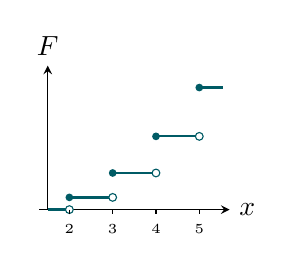
\begin{tikzpicture}[x=.55cm,y=1.55cm,>=stealth]
\draw[->] (1.3,0)--(5.7,0) node[right]{$x$};
\draw[->] (1.5,0)--(1.5,1.18) node[above]{$F$};
\draw[thick,accent] (1.5,0)--(2,0) (2,.1)--(3,.1) (3,.3)--(4,.3) (4,.6)--(5,.6) (5,1)--(5.55,1);
\foreach \x/\y in {2/.1,3/.3,4/.6,5/1}{\fill[accent] (\x,\y) circle (1.4pt);}
\foreach \x/\y in {3/.1,4/.3,5/.6}{\draw[accent,fill=white] (\x,\y) circle (1.4pt);}
\draw[accent,fill=white] (2,0) circle (1.4pt);
\foreach \x in {2,3,4,5}{\draw (\x,0)--(\x,-.04) node[below]{\tiny\x};}
\end{tikzpicture}\\[-2pt]
{\fontsize{7}{8}\selectfont Discrete maximum CDF}
\end{minipage}\hfill
\begin{minipage}{.48\linewidth}\centering
\begin{tikzpicture}[x=.43cm,y=1.55cm,>=stealth]
\draw[->] (-.35,0)--(6.75,0) node[right]{$x$};
\draw[->] (0,0)--(0,1.18) node[above]{$F$};
\draw[thick,accent] (0,0)--(2,.5)--(4,.5)--(6,1)--(6.55,1);
\foreach \x in {2,4,6}{\draw (\x,0)--(\x,-.04) node[below]{\tiny\x};}
\end{tikzpicture}\\[-2pt]
{\fontsize{7}{8}\selectfont Gap-density CDF}
\end{minipage}
\end{center}

\vfill
{\color{ink}\hrule height .35pt}\vspace{2pt}
{\fontsize{7}{8}\selectfont Sources: Freund, 8th ed., Ch. 3; Ross, 8th ed., pp. 168--170 (CDF endpoints).}
\end{multicols*}
\end{document}
